\documentclass[a4paper,10pt]{report}
\usepackage[frenchb]{babel}
\usepackage[utf8]{inputenc}
\usepackage[T1]{fontenc}
\usepackage{graphicx}
\usepackage{mathenv}
\usepackage{algpseudocode}
\usepackage{float}
\usepackage{hyperref}
\usepackage[final]{pdfpages} 
\usepackage{changepage}
\usepackage{graphicx}

\usepackage{array}

\usepackage{caption}

\usepackage[linesnumbered,ruled]{algorithm2e}

\usepackage{amssymb}

\newcounter{cnt}
\newcommand{\definition}{
  \addtocounter{cnt}{1}
 \textbf{Définition}
}



% Title Page
\title{Université d'Angers \\  \emph{M2 Intelligence Décisionnelle \\} \hrulefill \\ \textbf{Recherche de motifs fréquents par algorithmes évolutionnaires} \\ \hrulefill}
\author{Ugo Rayer}


\begin{document}

    \begin{titlepage}

\newcommand{\HRule}{\rule{\linewidth}{0.5mm}}

\center 

\textsc{\LARGE Université d'Angers}\\[1.5cm] 
\textsc{\Large M2 Intelligence Décisionnelle}\\ [0.5cm] 
\textsc{\large }\\[0.5cm] 


\HRule \\[0.4cm]
{ \huge \bfseries Recherche de motifs fréquents par algorithmes évolutionnaires}\\[0.4cm] 
\HRule \\[1.5cm]
 

\begin{minipage}{0.4\textwidth}
\begin{flushleft} \large
\emph{Auteur:}\\
Ugo \textsc{Rayer} 
\end{flushleft}
\end{minipage}
~
\begin{minipage}{0.4\textwidth}
\begin{flushright} \large
\hfill
\begin{tabular}{@{}l@{}}
\emph{Encadrants:}\\
Benoit \textsc{Da Mota} \\
Béatrice \textsc{Duval} \\
David \textsc{Lesaint} 
\end{tabular}
\end{flushright}
\end{minipage}\\[4cm]



{\large \today}\\[3cm] 




\includegraphics{./img/ua.jpg}\\[1cm]

\vfill 

\end{titlepage}

\newpage
~
\newpage
\chapter*{Remerciements}

Avant toute chose, je tiens à remercier l'ensemble des personnes qui ont participé, de près ou de loin, à la réalisation de ce stage et à l'écriture de ce rapport. \\

\hspace{0.2cm}Des remerciements spéciaux sont adressés d'une part au Laboratoire d'Etude et de Recherche en Informatique d'Angers pour son accueil et d'autre part au projet GRIOTE de la région Pays de la Loire qui a financé cette étude. Ensuite, je tiens à remercier chaleureusement Madame Duval et Messieurs Da Mota et Lesaint pour la qualité de leur encadrement et les différentes remarques qu'ils m'ont prodiguées pendant ces quelques mois. \\

\hspace{0.2cm}Enfin, un grand merci à Josépha pour ses précieux conseils d'écriture malgré l'incompréhension générale des sujets abordés.

\tableofcontents
\newpage

\chapter{Introduction}
Le calcul des motifs fréquents est une notion essentielle dans de nombreux domaines liés à la découverte et l'extraction de connaissances. Initiallement introduit par Agrawal et al. dans \cite{AGR93}, ces motifs étaient alors utilisés pour l'établissement de règles d'associations visant à caractériser les habitudes d'achats de clients d'un supermarché. Par exemple, une règle de la forme "Pain \& Beurre $\Rightarrow$ Jambon (75\%)" signifie que 3 clients sur 4 achetant du pain et du beurre achètent également du jambon. Le calcul de telles règles se fait en deux étapes, dont la principale (i.e. disposant de la plus grosse complexité calculatoire) correspond au calcul des motifs fréquents. Depuis son introduction, le problème du calcul des motifs fréquents a été très largement étudié et appliqué à de nombreux domaines comme en bio-informatique, en cybersécurité et bien évidemment en marketing.\\

\hspace{0.15cm}L'avènement de l'ère du Big Data a fait rentrer le problème de calcul des motifs fréquents dans une nouvelle dimension. En effet, le volume de données produites dans tous les domaines a cru de manière vertigineuse ces dernières années, rendant l'extraction de connaissances d'autant plus nécessaire et délicate. De fait, la problématique du passage à l'échelle des méthodes exactes est devenue primordiale. Bien que divers efforts en ce sens aient été faits au travers de nombreuses publications, ils se concentrent généralement sur l'optimisation et la parallélisation des méthodes existantes. \\

\hspace{0.15cm}Les algorithmes évolutionnaires font partie des techniques de résolution de problèmes combinatoires appelées méta-heuristiques. Les méta-heuristiques regroupent un ensemble de méthodes approchées à la résolution de problème combinatoire. Elles sont naturellement envisagée lorsque la complexité du problème étudié ne permet pas l'usage de méthodes exactes (aussi bien en temps qu'en espace). Le principe des algorithmes évolutionnaires est de manipuler un ensemble d'individus représentant chacun une solution au problème étudié. A chaque itération, certains individus sont modifiés via des opérateurs de croisement et de mutation. Chaque individu est évalué au regard d'une fonction à optimiser dépendant du problème étudié. \\

\hspace{0.15cm}Ainsi, nous formaliserons le problème de calcul de motifs fréquents dans la section suivante avant d'effectuer un état de l'art des méthodes existantes en section 3. Le chapitre 4 sera dédié à la présentation de notre méthode dont nous présenterons les résultats en section 5. Le dernier chapitre sera consacré à la conclusion de cette étude et à une ouverture vers de futurs travaux.

\newpage
\chapter{Le problème du calcul motifs fréquents}

\section{Définition du problème}
	La définition la plus courante du problème de calcul des motifs fréquents se fait par la théorie des ensembles. Nous verrons cependant dans le chapitre suivant qu'il peut également être décrit par la théorie des graphes. Nous présenterons dans un premier temps un cadre formel nécessaire à la définition du problème que nous illustrerons ensuite. Enfin, nous introduirons quelques propriétés dérivés de la définition du problème.

\subsection{Formalisation}
	Soit $\mathcal{I}$ un ensemble de \emph{symboles} appelées \textbf{items}. Quelque soit \emph{I} $ \subseteq \mathcal{I}$, \emph{I} est un \emph{motif} appelé \textbf{itemset}. \\

\hspace{0.15cm}Soit $\mathcal{T}$ = \{ \emph{$t_{1}$, ... , $t_{n}$ } \} un ensemble de \textbf{transactions}. Chaque élément \emph{$t_{i}$} est un couple $< tid, \emph{I} >$ où \emph{tid} est l'identifiant de la transaction et \emph{I} $\subseteq \mathcal{I}$. $\mathcal{T}$ est communément appelé \textbf{base de transactions}.  \\

\hspace{0.15cm}Pour tout itemset \emph{I} $\subseteq \mathcal{I}$ la \textbf{couverture} de \emph{I} par $\mathcal{T}$ est définie par : \\
\begin{center}
\textbf{cover$_{\mathcal{T}}$}(\emph{I}) = \{ \emph{t} $\in \mathcal{T}  | \emph{ I} \subseteq \emph{t }\}$
\end{center}

\hspace{0.15cm}La cardinalité de la couverture d'un itemset \emph{I} par $\mathcal{T}$ \\
\begin{center}
\textbf{sup$_{\mathcal{T}}$}(\emph{I}) = $|$ \textbf{cover$_{\mathcal{T}}$}(\emph{I}) $|$
\end{center}
est appelée \textbf{support} de \emph{I}.  Etant donné un support minimal \emph{minsup} l'ensemble des \textbf{itemsets} (i.e. motifs) \textbf{fréquents} est défini par : \\
\begin{center}
$\textbf{F}_{\mathcal{T},minsup}$ = \{ \emph{I} $\subseteq \mathcal{I } |$  $sup_{\mathcal{T}}(\emph{I}) \geq$ \emph{minsup} \}
\end{center}

\hspace{0.15cm}Le problème du \textbf{calcul des itemsets fréquents} ( \textbf{FIM} - \emph{Frequent Itemsets Mining}) est, étant donné une base de transactions $\mathcal{T}$ et un support minimal \emph{minsup} de calculer l'ensemble \emph{F} des itemsets fréquents. Comme F. Boden le remarque dans \cite{BOD06}, bien qu'historiquement définie comme une valeur relative et donc asujettie à un support minimal défini dans l'intervalle [0,1], le support est de nos jours mesuré de manière absolue. Si nécessaire, nous y ferons référence sous la notion de fréquence : \\
\begin{center}
$\textbf{Freq}_{\mathcal{T}}$(\emph{I}) = $\frac{ | \textbf{ cover$_{\mathcal{T}}$}(\emph{I})  | } { | \mathcal{T} | }$
\end{center}
avec \emph{minfreq} simplement définie par $\frac{\emph{minsup}}{| \mathcal{T} |}$. \\

\subsection{Exemple}
	Situons nous dans le contexte de la définition historique de problème et considérons la base de transactions suivante (que nous conserverons tout au long de cet article). Le tableau 1 décrit chaque transaction par : un identifiant, une liste d'objets achetés et la liste des items fréquents vis à vis d'un support minimal de  3.\\

\begin{tabular}{|c|l|l|}
	\hline
	ID transaction & Objets achetés & Items Fréquents Ordonnés \\
	\hline
	100 & f, c, a, d, g, i m, p & f, c, a, m, p \\
	\hline
	200 & a, b, c, f, l, m, o & f, c, a, b, m \\
	\hline
	300 & b, f, h, j, o & f, b \\
	\hline
	400 & b, c, k, s, p & c, b, p \\
	\hline
	500 & a, f, c, e, l, p, m, n & f, c, a, m, p \\
	\hline	
\end{tabular}
\captionof{table}{Base de transactions exemple}
\vspace{0.4cm}

\hspace{0.15cm}Une fois calculé, l'ensemble des itemsets fréquents vis à vis de ce jeu de données $\mathcal{T}$ est l'ensemble $\textbf{F}_{\mathcal{T},3}$ = \{ (f:4), (c:4), (a:3), (b:3), (m:3), (p:3), (fc:3), (fa:3), (fm:3), (cm:3), (cp:3), (ca:3), (am:3), (fca:3), (fcm:3), (fam:3), (cam:3), (fcam:3) \}.  \\

\subsection{Complexité et Propriétés}
La complexité du problème vient d'une part du nombre d'itemsets à considérer en fonction du nombre d'objets et d'autre part de nombre de transactions dans la base. En effet, soit \emph{n} objets fréquents dans la base, il y a alors $2^{n}$ itemsets possibles. D'autre part, le calcul du support d'un itemset se fait au travers de l'ensemble des transactions. L'efficacité d'une méthode à résoudre ce problème se fera donc par sa capacité à explorer intelligement l'espace des $2^{n}$ itemsets et par son efficacité à calculer le support d'un itemset vis à vis de $| \mathcal{T} |$. \\
\hspace{0.15cm}Différents théorèmes et propriétés issus de l'étude de ce problème sont utilisés dans les méthodes proposées pour le résoudre. Nous présentons les propriétés liées à la monotonie du support d'un ensemble et renvoyons le lecteur vers \cite{BOD06} et \cite{GOE} pour plus de détails. \\
\textbf{Monotonie du support.} Soit une base de transactions $ \mathcal{T} sur \mathcal{I} $ et soient \emph{X, Y} $\subseteq \mathcal{I}$ deux itemsets. Alors, \\
\begin{center}
\emph{X} $\subseteq $ \emph{Y} $\Rightarrow$ \textbf{sup$_{\mathcal{T}}$}(\emph{Y}) $ \leq $ \textbf{sup$_{\mathcal{T}}$}(\emph{X})
\end{center}

Cette propriété nous permet de dire que si un k-itemset \emph{X} (i.e. un itemset comprenant k objets) est fréquent, alors l'ensemble \emph{Y} des k-1-itemsets $\subset $\emph{X} est fréquent. Par exemple, (fca:3) est fréquent, de même que (fc:3), (fa:3) et (ca:3). Nous pouvons de manière duale dire que si un k- itemset \emph{X} est non-fréquent, alors aucun des k+1-itemset \emph{Y} tel que \emph{X} $ \subset $ \emph{Y} n'est fréquent. Ces deux observations sont à la base des différents sens de parcours de l'espace de recherche des $2^{n}$ itemsets possibles dans la plupart des algorithmes.

\section{Problème des itemsets clos maximaux}

	Afin de réduire l'espace de recherche, il a été proposé de contraindre la recherche à l'ensemble des itemsets clos. Un k-itemset\emph{X} fréquent est clos si \textbf{sup$_{\mathcal{T}}$}(\emph{X}) $>$ \textbf{sup$_{\mathcal{T}}$}(\emph{Y}) $ \forall  $ \emph{Y} tel que \emph{X} $ \subset $ \emph{Y}.  Un itemset clos est maximal si aucun de ses surensembles n'est fréquent. Ainsi dans notre exemple, l'ensemble des itemsets clos est   $\textbf{C}_{\mathcal{T},3}$ = \{ (f:4), (c:4), (b:3), (cp:3), (fcam:3) \} et l'ensemble des itemsets clos maximaux est  $\textbf{MC}_{\mathcal{T},3}$ =  $\textbf{C}_{\mathcal{T},3} - $ \{ (f:4), (c:4) \}. La figure suivante représente le treillis complet des différents itemsets possibles sur les objets fréquents. Y figurent d'une part les itemsets fréquents en vert, d'autre part les itemsets clos en jaune et enfin les itemsets clos maximaux en rouge. Pour plus de lisibilité, les itemsets non-fréquents ne figurent pas dans le treillis.\\

\begin{figure}
	\begin{adjustwidth}{-2.7cm}{}
	\begin{tabular}{l}
	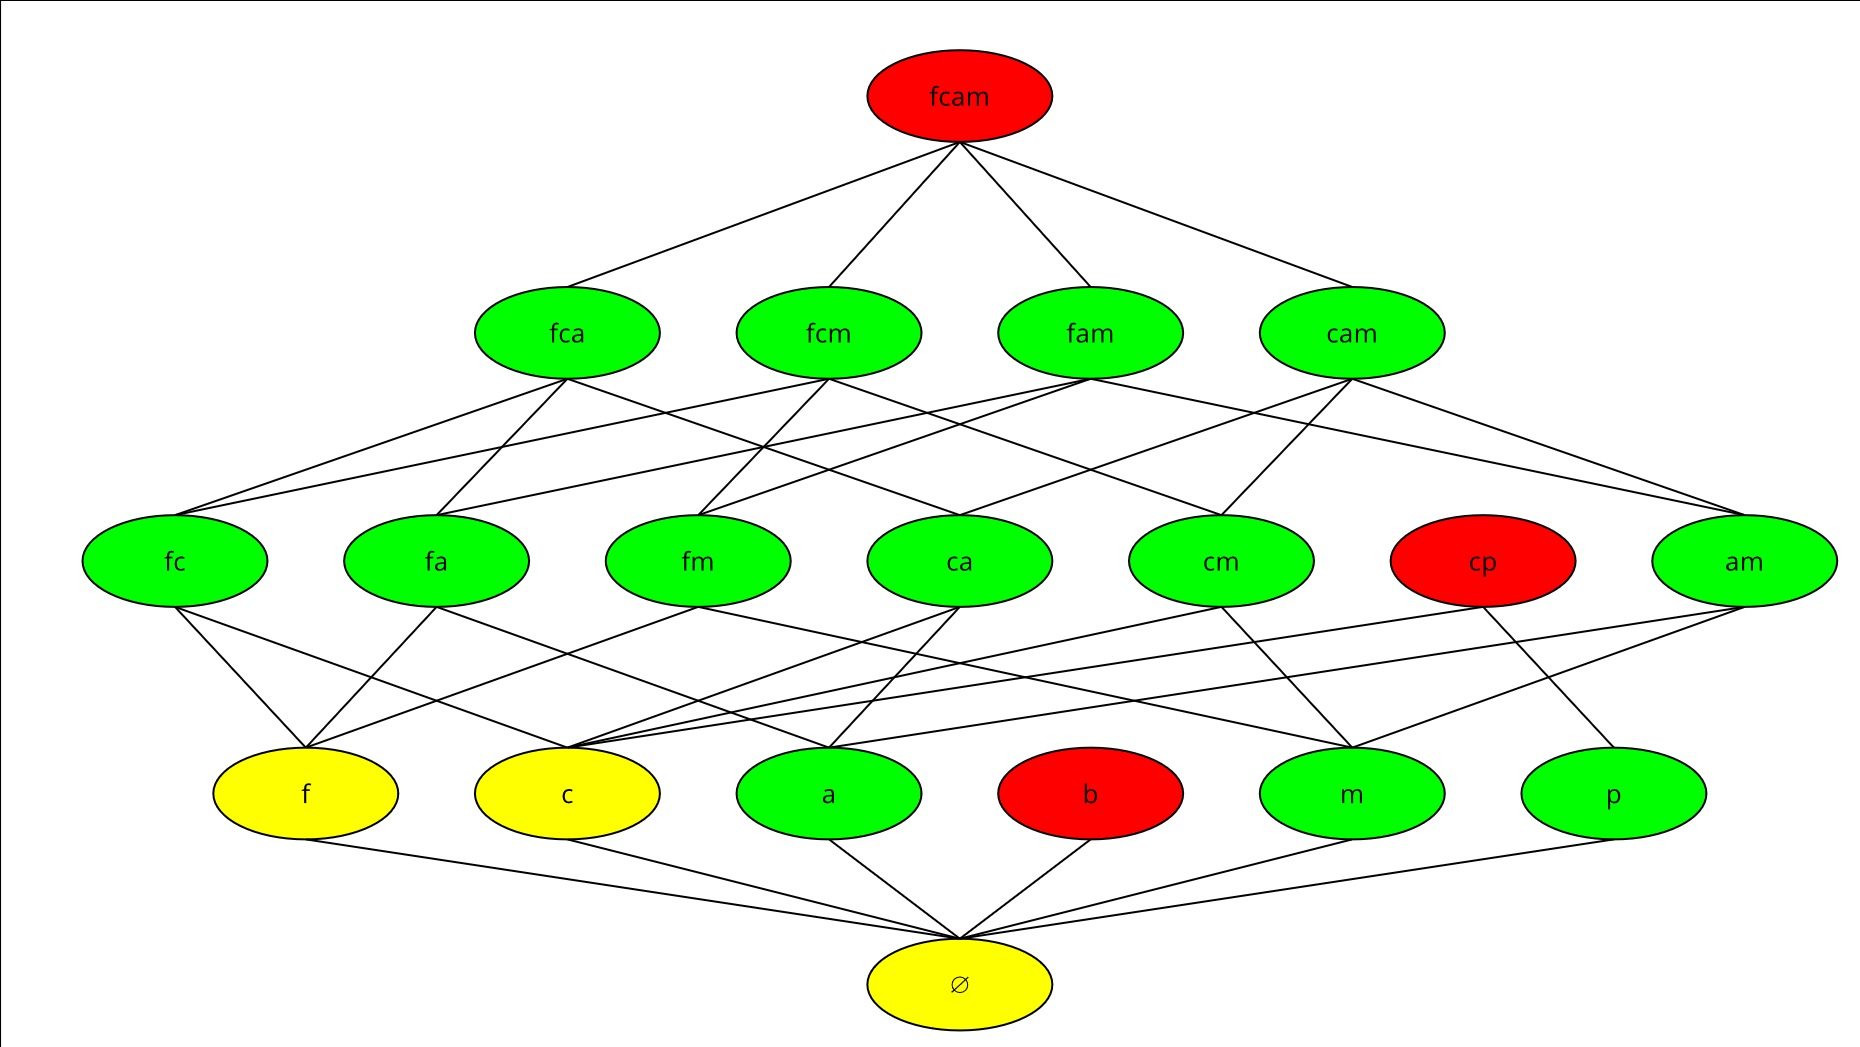
\includegraphics[width=15cm,height=12cm]{./img/treillis_is.jpg}\\
	\end{tabular}
	\caption{\label{fig:text}Treillis des itemsets fréquents, clos et maximaux de notre exemple}
	\end{adjustwidth}
\end{figure}

Zaki et al. et Pas. et al. prouvent dans \cite{ZAK99} et \cite{PAS99} que l'intégralité des itemsets fréquents peut être dérivée de l'ensemble des itemsets clos maximaux. Ils proposent alors d'adapter les méthodes existantes pour le calcul des itemsets clos maximaux. \\

\chapter{Etat de l'art}
\hspace{0.15cm}Dans ce chapitre, nous nous attacherons à présenter les principales méthodes de la littérature pour le calcul des itemsets fréquents. La première section sera dédiée à la présentation des méthodes exactes. Nous y aborderons les trois principaux algorithmes que sont A Priori \cite{AGR94}, Eclat \cite{ZAK00} et FP-Growth \cite{HAN04}. D'autres méthodes dédiées au calcul des itemsets clos maximaux seront également abordées. Enfin nous introduirons quelques méthodes présentant un intérêt pour la problématique du passage à l'échelle. La section 2 sera consacrée aux méthodes métaheuristiques de la littérature. [TO COMPLETE ] \\

\section{ Méthodes exactes}

\subsection{A Priori}

\hspace{0.15cm}Un an après avoir introduit le problème des règles d'associations (et par conséquent le problème de calcul des itemsets fréquents) dans \cite{AGR93}, les auteurs ont proposé l'algorithme A Priori \cite{AGR94} restant la référence littéraire du domaine. Son principe général est la génération de k+1-itemsets candidats à partir des k-itemsets fréquents précédemment calculés. L'algorithme 1 présente la phase de calcul des itemsets fréquents par A Priori. Nous ne présenterons pas l'algorithme calculant les règles d'associations dans cette étude. \\ 


\begin{algorithm}[H]
\caption{APriori Itemset Mining}
\SetKwInOut{Input}{Input}

\SetKwInOut{Output}{Output}
\Input{ $\mathcal{T}, \emph{minsup}$ }
\Output{ $\textbf{F}_{\mathcal{T},minsup}$ }
\Begin{
	
	$\emph{C}_{1}$ = \{ \{ \emph{i} \} $| \in \mathcal{I}$ \} \\
	\emph{k} = 1 \\
    \While{ $\emph{C}_{\emph{k}} \neq \{ \}$ } {
	// Calcul du support de chaque itemset candidat \\
        	\ForAll{ \emph{t} = ( \emph{tid, I} ) $ \in \mathcal{T} $ }{
		\ForAll{itemset candidat \emph{X} $\in \emph{C}_{k}$ } {
			\If{ \emph{X} $\subseteq$ \emph{I} }{
				\emph{X.support }++ \\
			}
		}
	}
	// Extraction de l'ensemble des itemsets fréquents \\
	$\textbf{F}_{\emph{k} } = \{ \emph{X } | \emph{ X.support} \geq \emph{minsup} \} $ \\
	// Génération des candidats de taille k+1 \\
	\ForAll{ \emph{X, Y} $\in \textbf{F}_{\emph{k}} | $ \emph{X}[i] = \emph{Y}[i] $\forall i \in [1,k-1] \& \emph{ X}[k] < \emph{Y}[k]  $ }{
		\emph{I} = \emph{X} $\cup$  \{ \emph{Y}[k] \} \\
		\If{ $\forall \emph{J} \subset \emph{I}, | \emph{J}| = \emph{k}$ et \emph{J} $\in \textbf{F}_{\emph{k}} $ }{
			$\emph{C}_{\emph{k+1}} =  \emph{C}_{\emph{k+1}} \cup \emph{I}$ \\

		}
	}
        
	\emph{k} ++
    }

}

\end{algorithm}

\hspace{0.15cm}Comme nous pouvons le constater, l'algorithme considère dans un premier temps l'ensemble des items comme candidats avant d'effectuer un premier scan de la base $\mathcal{ T }$ . Les 1-itemsets retenus sont utilisés pour générer des candidats de taille 2. L'algorithme poursuit cette routine jusqu'à ce qu'aucun candidat ne soit généré. \\

\hspace{0.15cm}Différentes implémentations efficaces ont été proposées pour améliorer la rapidité et l'espace mémoire nécessaire à l'exécution de l'algorithme Apriori. En général, les optimisations sont basées sur l'utilisation de structures spécifiques pour la représentation de la base de transactions et des itemsets candidats. Par exemple, \cite{BRI97} utilise un arbre préfixe pour stocker les itemsets candidats. D'autres structures incluant des vecteurs, des arbres de hachage et des structures hybrides existent également.\\

\hspace{0.15cm}Enfin, nous pouvons également mentionner l'existence d'implémentations d'Apriori utilisant le paradygme de la programmation parallèle. Par exemple \cite{YE06} présente une méthode parallèle partitionnant la base de transactions en sous-bases chacune assignée à un processeur différents. Une fois le calcul des k-itemsets localement fréquents, les résultats sont transmis à un noeud maître effectuant une centralisation des résultats. Notons également l'emploi de vecteurs pour stocker les 1 et 2-itemsets puis un arbre préfixe ensuite. \\

\subsection{Eclat}

\hspace{0.15cm}A la différence d'Apriori, qui effectue un parcours du treillis des candidats en largeur, Eclat est le premier algorithme à utiliser une représentation verticale de la base de transactions pour effectue une recherche en profondeur. Ainsi, Zaki et al. ont proposé cet algorithme dans \cite{ZAK00} en même temps que divers autres algorithmes dont certains basés sur une relation de pseudo-equivalence de cliques maximales.  \\

\hspace{0.15cm}Le tableau suivant  illustre la base de transactions utilisées dans l'exemple précédent représentée verticalement. Ainsi, nous ne traitons plus une liste d'items par transaction, mais une liste d'identifiants de transaction par item. Une telle liste est appelée \emph{tid-list}. De plus, Eclat utilise la notion de classe d'équivalence pour distribuer le calcul des itemsets candidats sur différents processeurs. Par exemple, les itemsets \emph{ABC} et \emph{ABD} appartiennent à la même classe d'équivalence $\mathcal{E}_\emph{AB}$.

\begin{center}

\begin{tabular}{|c|l|}
	\hline
	Item & \emph{tid-lists} \\
	\hline
	f & 100 200 300 500 \\
	\hline
	c & 100 200 400 500 \\
	\hline
	a & 100 200 500\\
	\hline
	b & 200 300 400 \\
	\hline
	m & 100 200 500 \\
	\hline
	p & 100 400 500\\
	\hline
\end{tabular}
\captionof{table}{Base de transactions verticale}

\vspace{0.4cm}
\end{center}

L'algorithme 2 présente la structure générale de l'algorithme Eclat. Le principe général est une recherche en profondeur d'abord calculant pour chaque item fréquent l'ensemble des itemsets le contenant. Un \emph{k+1}-itemset candidat est généré à partir de deux \emph{k}-itemsets partageant un même préfixe de taille \emph{k-1} et son support est calculé par l'intersection des \emph{tid-lists} des deux \emph{k}-itemsets. Dans le but de réduire le nombre de candidats générés, il est important de noter l'ordonnancement des items par support croissant.

\begin{algorithm}[H]
\caption{Eclat}
\SetKwInOut{Input}{Input}
\SetKwInOut{Output}{Output}
\Input{ $\mathcal{T}, \emph{minsup} , \emph{I} \subseteq \mathcal{I} $ (préfixe, initiallement $\emptyset$ ) }
\Output{ $\textbf{F}[\emph{I}](\mathcal{T},minsup) $= ensemble des k-itemsets fréquents partageant le même préfixe \emph{I} }
\Begin{
	$\textbf{F}[\emph{I }] = \emptyset $ \\
	\ForAll{ $\emph{i} \in \mathcal{T}$ }{
		$\textbf{F}[\emph{I }] $ = $\textbf{F}[\emph{I }] \cup \{ \emph{I} \cup \{i\} \}$ \\
		// Création des candidats de taille $|\emph{I }| + 1$ \\
		$\mathcal{D}^{i} = \emptyset $ \\
		\ForAll{$ \emph{j} \in \mathcal{ T } | \emph{j} > \emph{i}$ }{
			C = \emph{tid-list}[\{i\}] $\cap$ \emph{tid-list}[\{j\}] \\
			\If{ $|C| > \emph{minsup}$ }{ 
				$\mathcal{D}^{i} = \mathcal{D}^{i} \cup \{ (\emph{j}, C) \} $ \\
			}
		}
	// Récursion en profondeur sur \emph{i} \\
	Calculer $\textbf{F}[\emph{I } \cup \{\emph{i}\}](\mathcal{D}^{i}, \emph{minsup}$ ) \\
	$\textbf{F}[\emph{I }] = \textbf{F}[\emph{I }] \cup \textbf{F}[\emph{I} \cup \{\emph{i}\}] $\\
	}
}

\end{algorithm}

Sur notre exemple, l'algorithme Eclat extrairait dans un premier temps les itemsets contenant l'item \emph{p}, puis ceux contenant \emph{m} mais non \emph{p} etc. La propriété de monotonie du support n'est pas totalement employée puisqu'un itemset n'est pas candidat à condition que l'intégralité des ses sous-ensembles soient fréquents mais uniquement 2. Diverses améliorations ont été proposées dont une par les auteurs originels d'Eclat introduisant la notion de \emph{diffset} utilisée pour le calcul du support d'un itemset candidat. Références et détails sont disponibles dans \cite{GOE}. \\

\subsection{FP-Growth}

\hspace{0.15cm}Le dernier des 3 algorithmes les plus répandus et étudiés de la littérature est l'algorithme FP-Growth. Proposé par Han et al. dans \cite{HAN04}, il est également basé sur un parcours en profondeur item après item. Toutefois, il utilise une structure de données particulière, FP-Tree, permettant de condenser la base de transactions et d'en extraire diverses informations supplémentaires (distribution des items, bases conditionnelles de motifs...). Dans un premier temps nous introduirons la structure de FP-Tree en construisant celui associé à notre base de transactions exemple.

\subsubsection{Structure FP-Tree}

\hspace{0.15cm}Un FP-Tree est un arbre de préfixes construit à partir d'une base de transactions $\mathcal{T }$ et un support minimum \emph{minsup}. La construction d'un tel arbre se fait via deux scans de la base $\mathcal{T}$. Le premier permet de calculer $\mathcal{L}_{FI}$ = \{ (\emph{i}, C)$ | \emph{i} \in \mathcal{I}$ et C = \textbf{$sup_{\mathcal{T}}$}(\emph{\{i\}}) \}. \\
Cette liste est ensuite ordonnée par support décroissant. Sur notre exemple, le premier scan de $\mathcal{T}$ nous donne la liste suivante : \\
\begin{center}
	$ \mathcal{L}_{FI}$ = \{ (\emph{f}, 4), (\emph{c}, 4), (\emph{a}, 3), (\emph{b},3 ), (\emph{m}, 3), (\emph{p}, 3) \} \\
\end{center}

La seconde étape va nous permettre via cette liste de construire l'arbre de préfixe T de la manière suivante. Premièrement, un noeud null correspondant à la racine de l'arbre, de même qu'une header-table comprenant pour chaque item son label, le support de l'1-itemset qu'il induit et un pointeur vers le premier noeud de l'arbre portant le même label (initialisé à null). Un récapitulatif de cette première étape est visuellement présenté dans la figure suivante. \\

\begin{figure}
	\begin{adjustwidth}{-1cm}{}
	\begin{tabular}{l}
	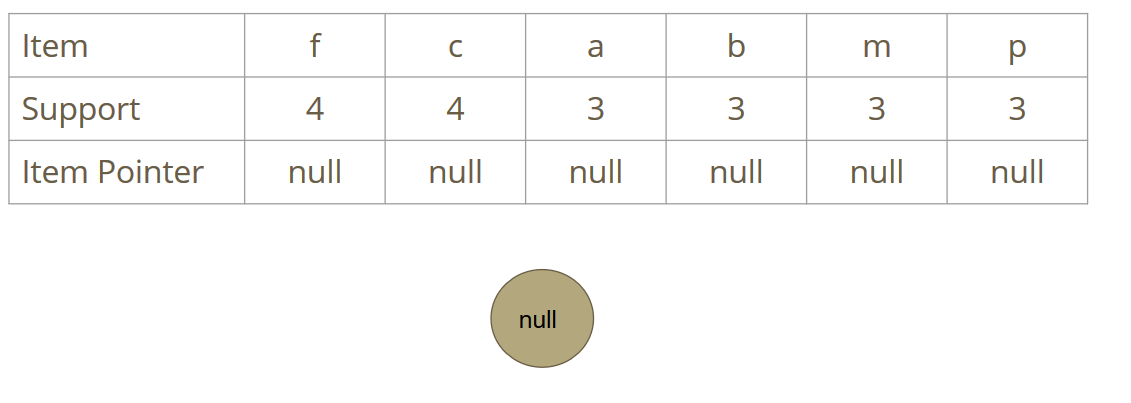
\includegraphics[width=15cm,height=5cm]{./img/fptree_init.jpg}\\
	\end{tabular}
	\caption{\label{fig:text}FP-Tree T après initialisation}
	\end{adjustwidth}
\end{figure}

Ensuite, chaque transaction \emph{t} de la base $\mathcal{T}$ est de nouveau scannée. Soit $[ p | P ]$ la liste des items \emph{i} $\in$ \emph{t} où p est le premier item et P le reste de la liste. Un noeud de l'arbre possède les informations suivantes : un label, un compteur, un pointeur vers son père et une liste de pointeurs vers ses noeuds fils. La fonction d'insertion de $[ p | P ]$  dans T est alors appelée et fonctionne comme suit. Si T fonctionne un fils N tel que le label de N soit le même que le label de p, alors on incrémente simplement le compteur de N de 1. Sinon, nous créons N avec un compteur initialisé à 1 et ayant T pour parent. On relie ensuite le dernier pointeur de la header-table correspondant au label de p à ce nouveau noeud N. Pour terminer, si P (le reste de la liste des items fréquents dans la transaction \emph{t}) est non vide, on appelle récursivement cette fonction avec P et N en paramètres. \\
Le processus est explicité dans la figure suivante présentant l'évolution du FP-Tree après lecture des deux premières transactions et après l'intégralité de la base. \\

\begin{figure}
	\begin{adjustwidth}{-4cm}{}
	\begin{tabular}{l}
	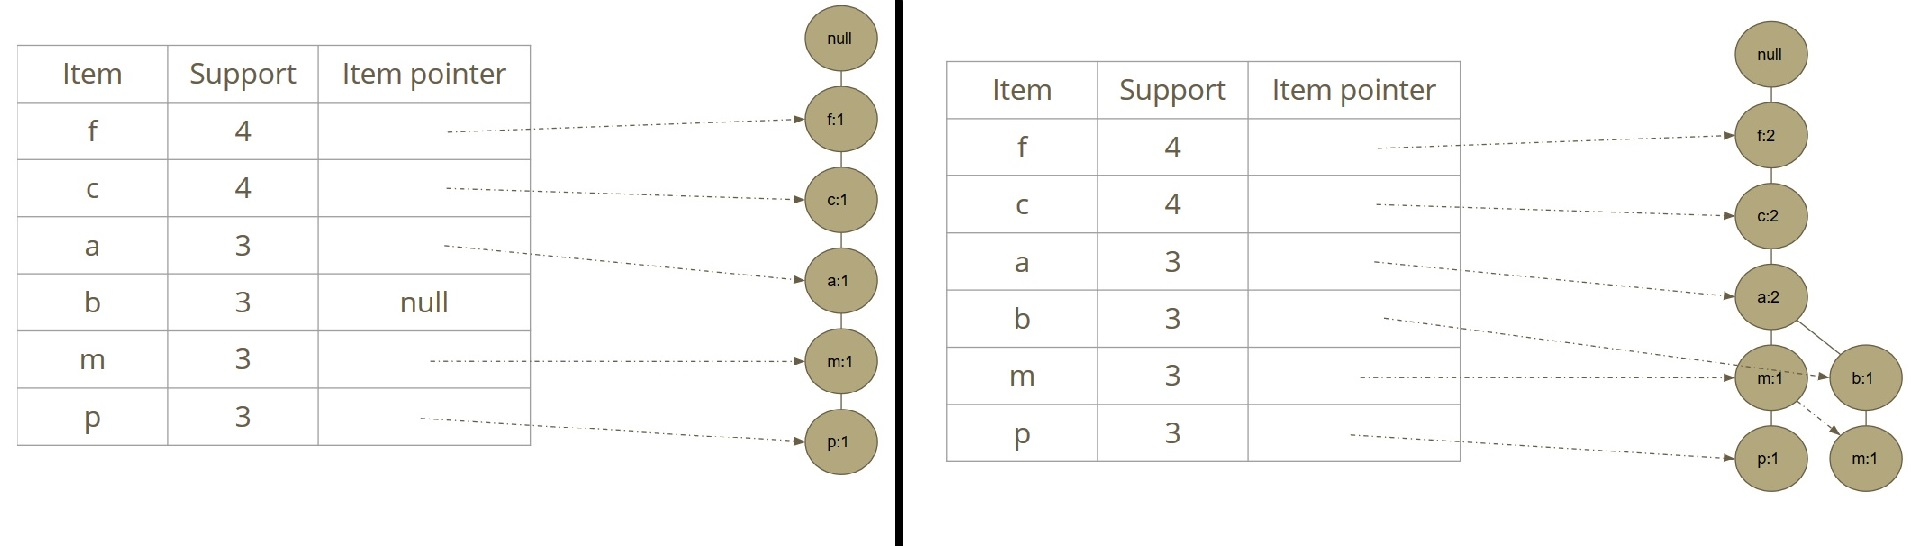
\includegraphics[width=20cm,height=8cm]{./img/t1.jpg}\\
	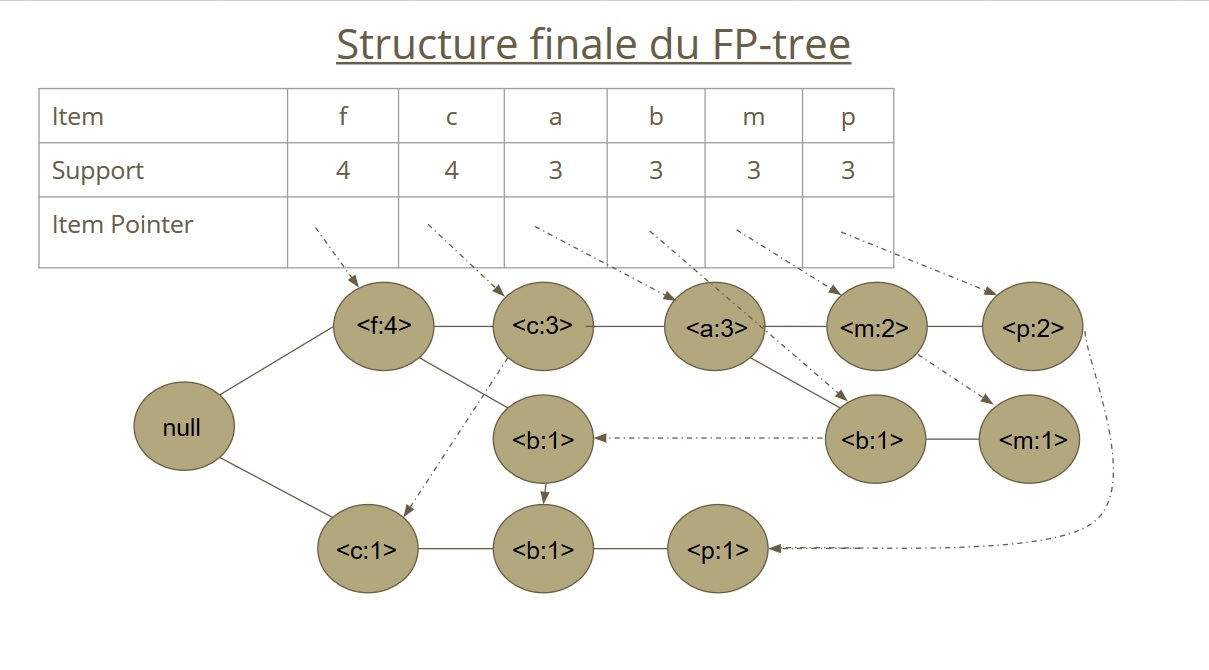
\includegraphics[width=20cm,height=8cm]{./img/fp_tree.jpg}\\
	\end{tabular}
	\caption{\label{fig:text}FP-Tree T après t1 et t2 et FP-Tree final}
	\end{adjustwidth}
\end{figure}

\newpage
\subsubsection{Extraction des itemsets fréquents}
\hspace{0.15cm}Une fois le FP-Tree obtenu à partir de $\mathcal{T}$, l'extraction des itemsets fréquents se fait de manière récursive en profondeur d'abord sur chacun des 1-itemsets contenus dans la header-table. Le principe d'augmentation de motif décrit est basé sur le calcul de base conditionelle de motifs depuis le FP-Tree. Le processus récursif se fait via le calcul de nouvelles bases conditionnelles sur les motifs venant d'être augmenté via la création de FP-Tree conditionnel sur ces bases. \\

La base conditionnelle d'un itemset $\emph{I}_{1}...\emph{I}_{k}$ correspond à l'ensemble des chemins du FP-Tree où l'itemset apparaît. L'algorithme traite les 1-itemsets de la header table du moins fréquent au plus fréquent et calcule pour chacun l'ensemble des itemsets fréquents le contenant. Le calcul de cette base conditionnelle se fait grâce à  la propriété suivante : \\

\emph{Pour chaque item fréquent $a_{i}$, l'ensemble des motifs contenant uniquement des items fréquents et $a_{i}$ peut être obtenu en suivant les noeuds-liens de $a_{i}$ en commençant par le noeud de la header-table.} \\

Sur notre exemple, l'extraction des itemsets fréquents commence avec l'item \emph{p}. En suivant les liens de la header-table pour l'item \emph{p}, nous pouvons extraire deux chemins le contenant (f:4, c:3, a:3, m:2, p:2) et (c:1, b:1, p:1). N'apparaissant respectivement que deux et une fois avec \emph{p}, nous conservons donc les préfixes (fcam:2) et (cb:1) qui forment la base conditionnelle de \emph{p}. La construction d'un FP-Tree sur cette base conditionnelle, appelé FP-Tree conditionnel de \emph{p} et dénoté FP-Tree$|_{p}$, mène à la création d'un seul noeud (c:3) et par conséquent  seul l'itemset (cp:3) est dérivé. Ne pouvant construire de base conditionnelle sur FP-Tree$|_{p}$, la recherche associée à l'item \emph{p} est terminée et les deux itemsets fréquents le contenant sont (cp:3) et (p:3). \\
L'extraction des itemsets où figurent l'item \emph{m} est décrit dans la figure suivante. La base conditionnelle de\emph{m} mène à la construction d'un FP-Tree conditionnelle devant être exploité, enclenchant ainsi la récursion en profondeur. Il est toutefois important de noter que lors de la construction d'un tel arbre, les items doivent être ordonnés par fréquence décroissante du nombre de noeuds dans lequel ils figurent.

\begin{figure}
	\begin{adjustwidth}{-1cm}{}
	\begin{tabular}{l}
	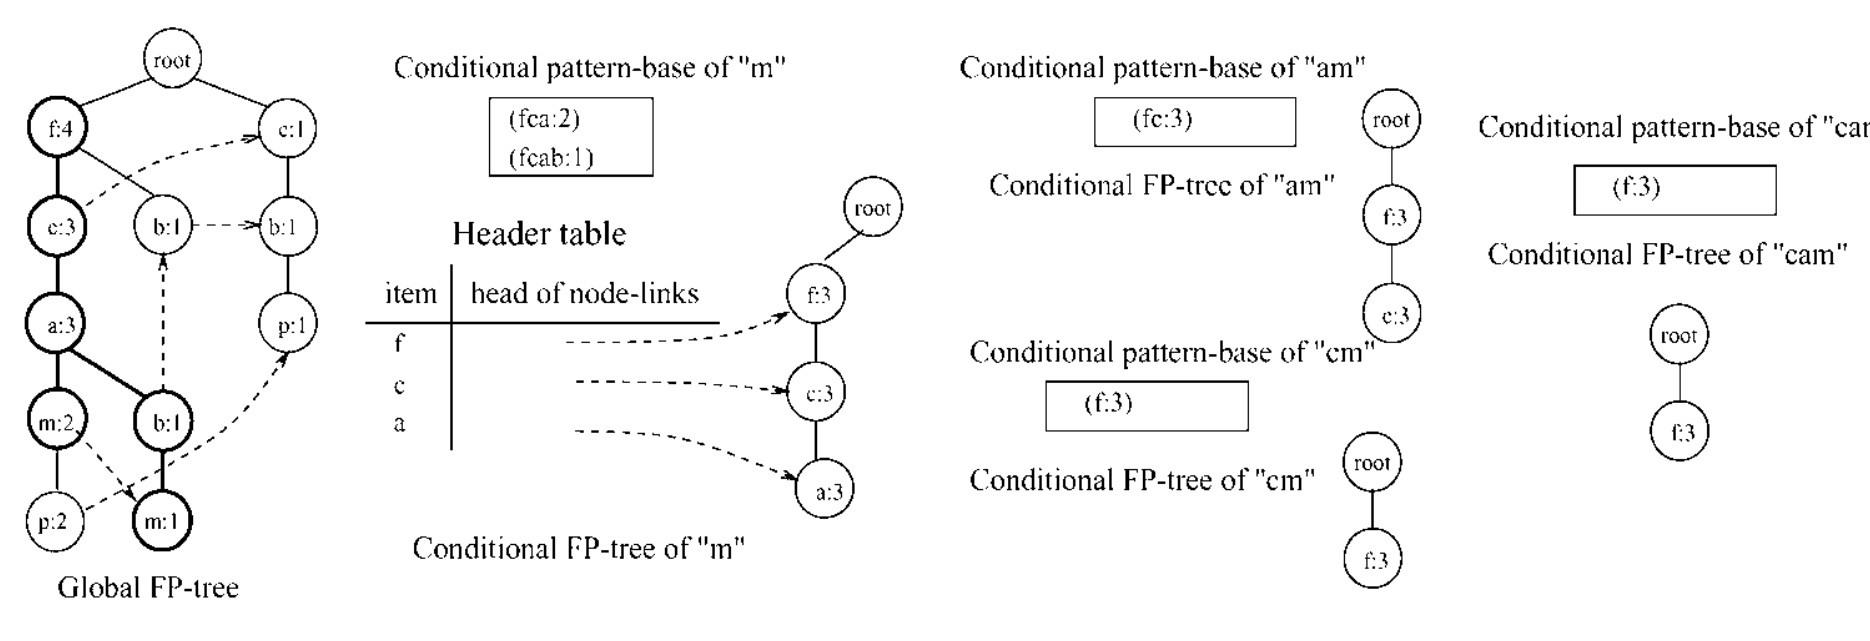
\includegraphics[width=15cm,height=7cm]{./img/mining_m}\\
	\end{tabular}
	\caption{\label{fig:text}Extraction des itemsets contenant \emph{m}}
	\end{adjustwidth}
\end{figure}

La génération des itemsets fréquents via la base conditionnelle d'un sous-motifs se fait grâce à la propriété suivante : \\

\emph{Soit $\alpha$ un itemset fréquent dans $\mathcal{T}$, soient $\mathcal{T}_{\alpha}$ la base conditionnelle de motifs d'$\alpha$ et $\beta$ un itemset $\in \mathcal{T}_{\alpha}$ Alors $\alpha \cup \beta$ est fréquent dans $\mathcal{T}$ si et seulement si $\beta$ est fréquent dans $\mathcal{T}_{\alpha}$}. \\

Différentes optimisations sont proposées pour accélérer le processus d'extraction. La principale et plus intéressante est liée à la topologie du FP-Tree. En effet, si celui-ci contient un seul chemin, alors l'ensemble des itemsets fréquents peut être obtenu en énumérant l'ensemble des combinaisons d'items le long de ce chemin avec pour support celui de l'item y appartenant ayant le plus faible. Sur notre exemple, nous aurions par exemple pu énumérer l'ensemble des combinaisons du FP-Tree$|_{m}$ pour en extraire l'intégralité des itemsets le contenant. Cette propriété a été étendue pour exploiter les arbres contenant un préfixe unique en considérant ce préfixe comme un chemin unique ( énumération des combinaisons) et la partie multiple comme un autre FP-Tree en ajoutant une racine au niveau de l'embranchement. Ainsi, l'extraction complète se fait par l'union des itemsets produit par l'énumération avec ceux produits par le processus récursif et enfin avec les itemsets obtenus par combinaisons d'éléments appartenant à l'un et l'autre des ensembles. \\

Bien qu'étant les trois références en matière de méthodes exactes pour l'extraction des itemsets fréquents, ces algorithmes ont malheureusement de nombreuses difficultés à être comparés. En effet, différentes optimisations et implémentations ayant été proposées, de nombreux articles de la littérature présentent des conclusions différentes sur l'efficacité des méthodes. Nous pouvons toutefois considérer que chaque algorithme possède des performances variables principalement selon les caractéristiques du jeu de données étudié et de la qualité de l'implémentation qui en est faite. Nous allons maintenant présenter rapidement quelques algorithmes pour la recherche des itemsets clos avant d'introduire les méta-heuristiques utilisées pour résoudre ce problème.

\subsection{Algorithmes pour itemsets clos}

De la même manière que trois algorithmes pour les itemsets fréquents ont été présentés, trois pour l'extraction des itemsets clos le seront également. Toutefois, nous serons plus succint et renverrons le lecteur au article correspondant quand nécessaire. Ainsi, nous présenterons rapidement les algorithmes A-Close (\cite{PAS99}), Charm (\cite{ZAK99})et Closet, utilisant également un FP-Tree pour fonctionner (\cite{PEI00}). \\

\subsubsection{A-Close}
\hspace{0.15cm}Proposé par Pasquier et al. en 1999 dans \cite{PAS99}, l'algorithme A-Close est l'adaptation d'A Priori  pour l'extraction des itemsets clos. Il est composé de deux phases. La première effectue une recherche bottom-up dans le but d'identifier l'ensemble des \emph{générateurs}, i.e. les plus petits itemsets qui déterminent un itemset clos via l'opérateur de clôture défini sur la correspondance de Galois entre itemsets et transactions. Le calcul des \emph{générateurs} se fait via une légère modification d'A Priori. En effet, à chaque fois qu'un ensemble de candidats est généré, A-Close calcule leur support et élimine l'ensemble des non-fréquents. Pour chaque itemset candidat restant, leur support est comparé à celui de ses sous-ensembles calculé au niveau précédent. Si le support d'un candidat égale celui d'un de ses sous-ensembles, cet itemset ne peut pas être un \emph{générateur} et est donc supprimé. Cette phase continue jusqu'à ce qu'aucun \emph{générateur} ne soit produit. \\

\hspace{0.15cm} La seconde phase de l'algorithme A-Close consiste, une fois l'ensemble des \emph{générateurs} obtenus, à calculer la clôture de chacun d'entre eux et à éliminer les redondances. Le calcul de la clôture d'un itemset se fait par l'intersection de l'ensemble des transactions dans lesquelles cet itemset apparaît. Ce calcul peut se faire via un seul scan du jeu de données sous réserve que l'intégralité des \emph{générateurs} tient en mémoire centrale.

\subsubsection{Charm}
\hspace{0.15cm} De la même manière qu'A-Close, Charm définit une correspondance de Galois entre les ordres partiels induits par les itemsets et les transactions. Toutefois, Charm explore simultanément l'espace des itemsets et celui des tidsets en effectuant des opérations d'union sur les premiers et d'intersection sur les seconds. L'algorithme construit l'arbre des itemsets clos fréquents via les quatre propriétés suivantes tout en élaguant dès que possible les itemsets non fréquents et non clos. \\

\textbf{Propriété 1} \\
Si \textbf{cover$_{\mathcal{T}}$}(\emph{$I_{1}$}) = \textbf{cover$_{\mathcal{T}}$}(\emph{$I_{2}$}) alors \textbf{cover$_{\mathcal{T}}$}(\emph{$I_{1}$} $\cup$ \emph{$I_{2}$}) = \textbf{cover$_{\mathcal{T}}$}(\emph{$I_{1}$})  $\cap$ \textbf{cover$_{\mathcal{T}}$}(\emph{$I_{2}$}) = \textbf{cover$_{\mathcal{T}}$}(\emph{$I_{1}$}) = \textbf{cover$_{\mathcal{T}}$}(\emph{$I_{2}$}). Dans ce cas, nous pouvons remplacer toutes les occurences de \emph{$I_{1}$} par \emph{$I_{1}$}$\cup$\emph{$I_{2}$} et retirer \emph{$I_{2}$} des considérations futures.\\

\textbf{Propriété 2} \\
Si \textbf{cover$_{\mathcal{T}}$}(\emph{$I_{1}$}) $\subset$ \textbf{cover$_{\mathcal{T}}$}(\emph{$I_{2}$}) alors \textbf{cover$_{\mathcal{T}}$}(\emph{$I_{1}$}  $\cup$ \emph{$I_{2}$}) = \textbf{cover$_{\mathcal{T}}$}(\emph{$I_{1}$})  $\cap$ \textbf{cover$_{\mathcal{T}}$}(\emph{$I_{2}$}) = \textbf{cover$_{\mathcal{T}}$}(\emph{$I_{1}$}) $\neq$ \textbf{cover$_{\mathcal{T}}$}(\emph{$I_{2}$}). Dans ce cas, nous pouvons remplacer toutes les occurentes de \emph{$I_{1}$} par \emph{$I_{1}$}$\cup$\emph{$I_{2}$} mais devons conserver \emph{$I_{2}$} dans les considérations futures puisque \textbf{cover$_{\mathcal{T}}$}(\emph{$I_{1}$}) $\neq$ \textbf{cover$_{\mathcal{T}}$}(\emph{$I_{2}$}). \\

\textbf{Propriété 3} \\
Si \textbf{cover$_{\mathcal{T}}$}(\emph{$I_{1}$}) $\supset$ \textbf{cover$_{\mathcal{T}}$}(\emph{$I_{2}$}) alors \textbf{cover$_{\mathcal{T}}$}(\emph{$I_{1}$}  $\cup$ \emph{$I_{2}$}) = \textbf{cover$_{\mathcal{T}}$}(\emph{$I_{1}$})  $\cap$ \textbf{cover$_{\mathcal{T}}$}(\emph{$I_{2}$}) = \textbf{cover$_{\mathcal{T}}$}(\emph{$I_{2}$}) $\neq$ \textbf{cover$_{\mathcal{T}}$}(\emph{$I_{1}$}). De la même manière que dans la propriété précédente, nous pouvons remplacer toutes les occurences de \emph{$I_{2}$} par \emph{$I_{1}$}$\cup$\emph{$I_{2}$} et conserver \emph{$I_{1}$} dans les futures considérations. \\

\textbf{Propriété 4} \\
Si \textbf{cover$_{\mathcal{T}}$}(\emph{$I_{1}$}) $\neq$ \textbf{cover$_{\mathcal{T}}$}(\emph{$I_{2}$}) alors \textbf{cover$_{\mathcal{T}}$}(\emph{$I_{1}$}  $\cup$ \emph{$I_{2}$}) = \textbf{cover$_{\mathcal{T}}$}(\emph{$I_{1}$})  $\cap$ \textbf{cover$_{\mathcal{T}}$}(\emph{$I_{2}$}) $\neq$ \textbf{cover$_{\mathcal{T}}$}(\emph{$I_{2}$}) $\neq$ \textbf{cover$_{\mathcal{T}}$}(\emph{$I_{1}$}). Dans ce cas, on ne peut rien éliminer car \emph{$I_{1}$} et \emph{$I_{2}$} ont des fermetures différentes. On peut en revanche ajouter le noeud \emph{$I_{1}$}$\cup$\emph{$I_{2}$} et son tidset associé \textbf{cover$_{\mathcal{T}}$}(\emph{$I_{1}$})  $\cap$ \textbf{cover$_{\mathcal{T}}$}(\emph{$I_{2}$}).

\subsubsection{Closet}
\hspace{0.15cm}L'algorithme Closet (\cite{PEI00}) est l'adaptation par ses auteurs de l'algorithme FP-Growth pour l'extraction des itemsets clos fréquents. En effet, il utilise différentes optimisations pour extraire rapidement des itemsets clos et ainsi réduire d'une part le nombre d'appels récursifs de FP-Growth et d'autre part de réduire l'espace mémoire total nécessaire. \\

\hspace{0.15cm}La première propriété utilisée prend effet avant la construction d'un FP-Tree sur une base conditionnelle. En effet, s'il existe un ensemble d'items \emph{Y} apparaissant dans chaque transaction de la base conditionnelle de l'itemset \emph{X}, alors \emph{X} $\cup$ \emph{Y} forme un itemset fréquent clos s'il n'est pas un sous-ensemble d'un itemset fréquent clos déjà trouvés. \\

\hspace{0.15cm}La seconde propriété permet d'extraire des itemsets fréquents clos directement depuis le FP-Tree en réutilisant le principe de chemin unique dans le FP-Tree.  Soit \emph{i} un item fréquent dans la base conditionnelle de l'itemset \emph{X}. Si \emph{i} ne possède qu'un noeud \emph{N} dans le FP-Tree$|$\emph{X} et chaque ancêtre de \emph{N} n'a qu'un enfant et que \emph{N} n'en a pas, plusieurs, ou un seul avec un support inférieur, alors le \emph{i-single segment itemset} est l'union de l'itemset \emph{X} et des items incluant \emph{N} et l'ensemble de ces successeurs. Le \emph{i-single segment itemset Y} est un itemset fréquent clos si le support de \emph{i} dans la base conditionnelle de \emph{X} passe le support minimal et que \emph{Y} n'est pas un sous-ensemble strict d'aucun des itemsets fréquents clos déjà trouvés. Cette propriété est explicitée dans la figure 3.4.\\

\hspace{0.15cm}Enfin, Closet utilise une stratégie pour élaguer l'espace de recherche via la dernière propriété. Soient \emph{X} et \emph{Y} deux itemsets avec le même support. Si \emph{X} $\subset$ \emph{Y} et que \emph{Y} est clos, alors il n'existe aucun itemset fréquent clos contenant \emph{X} mais pas \emph{Y}$\setminus$\emph{X}.

\begin{figure}
	\begin{adjustwidth}{-1cm}{}
	\begin{tabular}{l}
	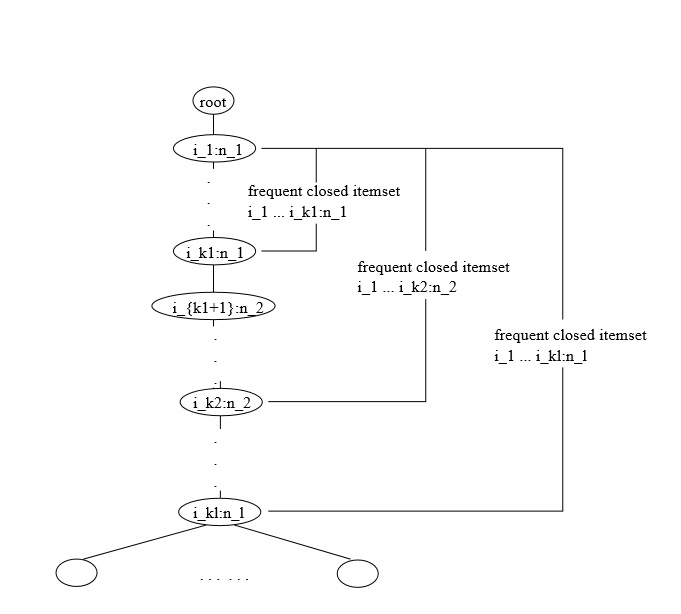
\includegraphics[width=15cm,height=8cm]{./img/closet_p2}\\
	\end{tabular}
	\caption{\label{fig:text}Extraction des itemsets fréquents clos depuis un FP-Tree}
	\end{adjustwidth}
\end{figure}	

\newpage
\section{Théorie des graphes}
	Le problème que nous étudions a également été défini comme un problème de calcul de cliques maximales dans un graphe biparti. \\
	
\subsection{Définition du problème}
	La base de transactions sur laquelle s'effectue la recherche des itemsets fréquents peut également être représentée par un graphe biparti. Un graphe est dit biparti s'il existe une partition de son ensemble de sommets en deux sous-ensembles \emph{U} et \emph{V} telle que chaque arête ait une extrémité dans \emph{U} et l'autre dans \emph{V}. Ce type de graphe permet notamment de représenter une relation binaire, ce qui est le cas de notre problème puisque la base de transactions est une relation binaire entre un ensemble d'items et un ensemble d'identifiants de transactions. \\
	
	Ainsi, soit le graphe biparti G = (U,V,E) tel que U = \{ $\emph{t}_{j}$ | $\emph{t}_{j} \in \mathcal{T}$ \}, V = \{ \emph{i} | \emph{i} $\in \mathcal{I}$ \} et E = \{ (u,v) | u $\in$ U, v $\in$ V et $\mathcal{T}_{u,v}$ = 1. Le problème d'extraction pouvant être ramené au calcul des itemsets fréquents clos maximaux (\cite{ZAK00}), nous pouvons le redéfinir selon cette représentation comme le calcul de l'ensemble des bicliques maximales. Une biclique est un graphe biparti complet, i.e. $\forall$ u $\in$ U et v $\in$ V, (u,v) $\in$ E. Une biclique G' = (U', V') obtenue depuis G est maximale si et seulement si $\not\exists$ U'' ou V'' | U' $\subset$ U'' $\subseteq$ U, V' $\subset$ V'' $\subseteq$ V tel que G''= (U'', V'') est complet. La figure 3.5 illustre notre base sous la représentation d'un graphe biparti ( format matriciel et graphique).\\
	
	Une procédure simple pour vérifier si un graphe biparti est complet consiste à calculer sa densité. En effet, un graphe biparti de densité 1 est complet. La densité d'un tel graphe G = (U, V, E) est défini par le ratio $\frac{|E|}{|U|*|V|}$. \\
	
\begin{figure}
	\begin{adjustwidth}{-1cm}{}
	\begin{tabular}{l}
	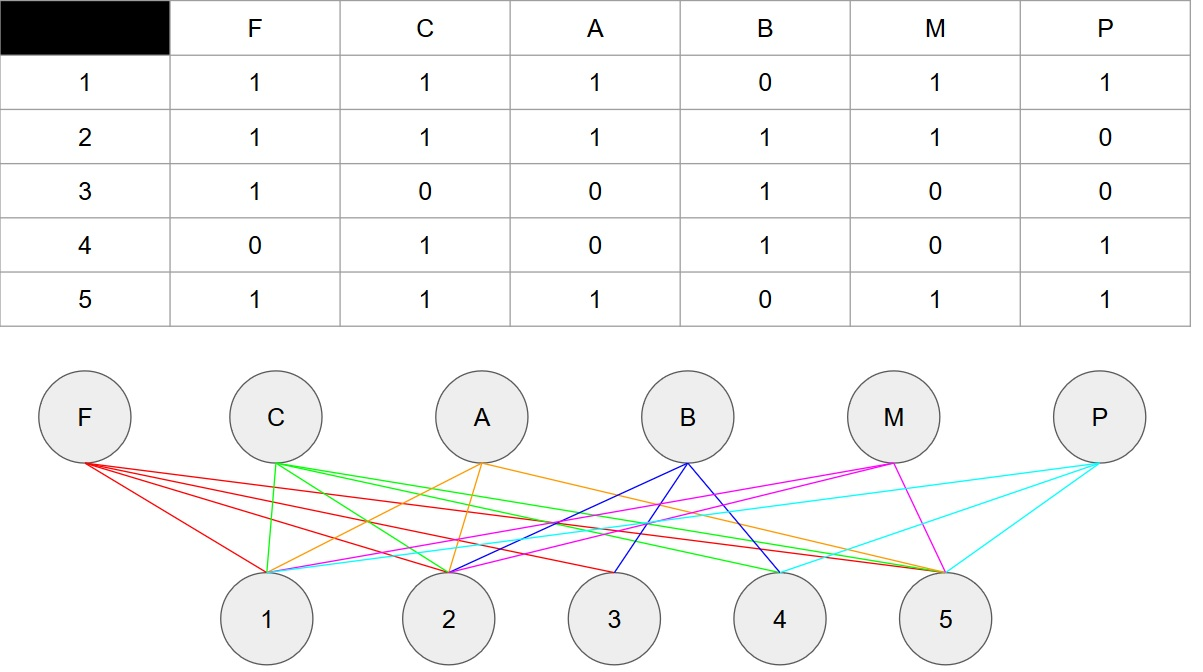
\includegraphics[width=15cm,height=8cm]{./img/graphe_biparti}\\
	\end{tabular}
	\caption{\label{fig:text}$\mathcal{T}$ représenté en graphe biparti}
	\end{adjustwidth}
\end{figure}

Le problème d'extraction de l'ensemble des motifs fréquents revient donc à calculer l'ensemble des bicliques $\mathcal{K}_{\delta, \omega}$ depuis G telles que $\delta \geq$ \emph{minsup}. \\


\subsubsection{Procédures}

	La procédure 1 décrit la construction du graphe biparti induit sur G par un itemset X passé en paramètre. La seconde permet de calculer le support de l'itemset décrit par le graphe induit calculé par la première procédure.
\begin{algorithm}[H]
\caption{Induced Graph of X}
\SetKwInOut{Input}{Input}

\SetKwInOut{Output}{Output}
\Input{ TDB $\mathcal{T}$, itemset \emph{X} }
\Output{ G'= (U', V', E') graphe induit par \emph{X} sur $\mathcal{T}$ }
\Begin{
	
	\ForAll{ x $\in$ \emph{X}}{
		V' = V' $\cup$ \{x\} \\
		\ForAll{ t $\in \mathcal{T}$}{
			\If{$\mathcal{T}[t][x]$ == 1}{
				U' = U' $\cap$ {t} \\
				E' = E' $\cup$ \{ (t,x) \} \\
			}
		}
	}
	\textbf{Return} \{ U', V', E' \} \\
}

\end{algorithm}


\begin{algorithm}[H]
\caption{Support Counting}
\SetKwInOut{Input}{Input}

\SetKwInOut{Output}{Output}
\Input{  G'= (U', V', E') graphe induit par \emph{X} sur $\mathcal{T}$  }
\Output{ Support de \emph{X} }
\Begin{
	supp = 0 \\
	\ForAll{ v $\in$ V'}{
		
		\If{$D_{v}$ == |U'|}{
			supp += 1 \\	
		}
		
	}
	\textbf{Return} supp \\
}

\end{algorithm}

\addcontentsline{toc}{chapter}{Bibliographie}
\bibliography{biblio}
\bibliographystyle{unsrt}

\end{document}